\documentclass[aspectratio=169,14pt,usenames,dvipsnames]{beamer}
\usetheme{TalentSprint}
\usepackage[utf8]{inputenc}
\usepackage{graphics}
\usepackage{ragged2e}
\usepackage{amsfonts}
\usepackage{xcolor}
\usepackage{mathtools}
\usepackage{tcolorbox}
\usepackage{setspace}
\usepackage{lmodern}
\usepackage{animate}
\definecolor{swe}{rgb}{0.19, 0.73, 0.56}
\definecolor{lgreen}{RGB}{190,200,198}
\title[Logistic Regression]{Logistic Regression}

\begin{document}

{\1
\begin{frame} \vspace{35pt}
	\maketitle
\end{frame}
}

\begin{frame}{Is it Classification or Regression}
\begin{itemize}
\item<2->  Logistic Regression is a supervised and classification Algorithm
\end{itemize}
\end{frame}

\begin{frame}{Why Logistic Regression called as "Regression"}
\begin{columns}
\begin{column}{0.55\textwidth}
\begin{itemize}
  \itemsep1em 
  \item In linear regression, a real-valued output y is predicted based on a weighted sum of input variables
  \item Whereas in Logistic regression, transforms its output using the logistic sigmoid function to return a probability value of 1 or 0.
\end{itemize}
\end{column}
\begin{column}{0.45\textwidth}
	\vskip-0.5cm
	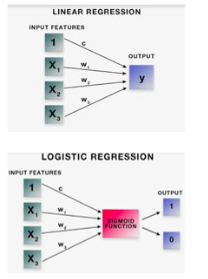
\includegraphics[width=0.7\textwidth, height=0.6\textheight]{Images/AIML_LR_IMG1.png}
\end{column}
\end{columns}
\end{frame}

\begin{frame}{Transform the model}
\begin{columns}
\column{0.6\textwidth}
\begin{itemize}
  \item Logistic Regression is a type of Generalized Linear Models.
\end{itemize}
\begin{itemize}
\item Output of the linear regression is passed through a sigmoid function that can map any real value between 0 and 1.
\end{itemize}
\column {0.5\textwidth}
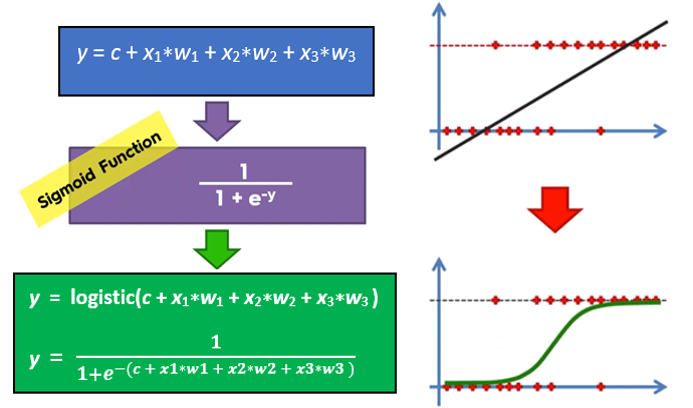
\includegraphics[width=0.9\textwidth, height=0.5\textheight]{Images/AIML_LR_IMG2.png}
\end{columns}
\end{frame}

\begin{frame}{ Know about Logistic Regression}
\begin{itemize}
  \item Predicts the categorical dependent variable using a given set of independent variables. 
\end{itemize}
\begin{itemize}
\item Predictive modeling.
\end{itemize}
\begin{itemize}
\item Uses a more complex cost function called as Sigmoid function or logistic function.
\end{itemize}
\begin{itemize}
\item Maps predicted values to probabilities which lie between 0 and 1.
\end{itemize}
\end{frame}

 
\begin{frame}{Decision Boundary}
\begin{columns}
\column{0.6\textwidth}
\begin{itemize}
  \item In this fig, A boundary line created by the classifier (Logistic Regression) signifies the decision regions.
\end{itemize}
\column {0.5\textwidth}
%\animategraphics {Images/AIML_LR_IMG3.gif}
\end{columns}
\end{frame}

\begin{frame}{Sigmoid Function}
\begin{columns}
\column{0.8\textwidth}
\begin{itemize}
  \item As you see in the graph, it is an S-shaped curve that gets closer to 1 as the value of input variable increases above 0 and gets closer to 0 as the input variable decreases below 0. The output of the sigmoid function is 0.5 when the input variable is 0.
\end{itemize}
\begin{itemize}
\item If the output is more than 0.5, we can classify the outcome as 1 (or positive) and if it is less than 0.5, we can classify it as 0 (or negative).
\end{itemize}
\column {0.4\textwidth}
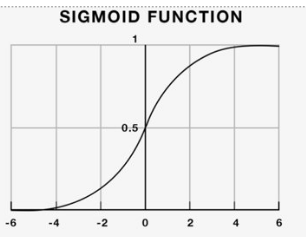
\includegraphics[width=0.7\textwidth, height=0.5\textheight]{Images/AIML_LR_IMG4.png}
\end{columns}
\end{frame}

\begin{frame}{Probability with Sigmoid Function}
\begin{itemize}
\item The transformation is defined as the logged odds:

- Odds = probability presence of the characteristic (P) /probability of absence of characteristic (1-P)

- Ln(P/(1-P) )= c + x1*w1 + x2*w2 + x3*w3 
\end{itemize}
\begin{itemize}
\item Being positive class over being negative class could be expressed as below for a binary classification task.

P(y = 1) / P(y = 0) 

P(y = 1) / (1 – P(y = 1)) 
\end{itemize}

\end{frame}


\begin{frame}{Types of Logistic Regression}
\small{Based on those number of categories, Logistic regression can be divided into following types :}
\begin{itemize}
\small {\item \textbf{Binary or Binomial} - dependent variable have only two possible types either 1 and 0.

- For example, these variables may represent success or failure, yes or no, win or loss etc.}
\end{itemize}
\begin{itemize}
\small {\item \textbf{Multinomial} - dependent variable can have 3 or more possible unordered types or the types having no quantitative significance. 

- For example, these variables may represent “Type A” or “Type B” or “Type C”.}
\end{itemize}
\end{frame}


\begin{frame}{Types of Logistic Regression}
\begin{itemize}
\small{\item \textbf{Ordinal} - dependent variable can have 3 or more possible ordered types or the types having a quantitative significance. }

- For example, these variables may represent “poor” or “good”, “very good”, “Excellent” and each category can have the scores like 0,1,2,3.
\end{itemize}
\end{frame}
	
\begin{frame}{Applications of Logistic Regression}
\begin{itemize}
\item Predicting a probability of a person having a heart attack
\item Predicting the probability of failure of a given process or product.
\item Predict whether a bank loan can be granted to a particular customer or not.
\item More….
\end{itemize}
\end{frame}

\begin{frame}{Demo Experiment}
\begin{itemize}
\item Demo Experiment on Logistic Regressions
- To find the logistic regression function p(x) such that the predicted responses p(x\_i) are as close as possible to the actual response.
\end{itemize}
\end{frame}

{ \1
\begin{frame}
	\title{Thanks!!}
	\subtitle{Questions?}
	\maketitle
\end{frame}
}

\end{document}
